\subsection{Dataset flor Iris}

Empezaremos importando las bibliotecas necesarias para realizar esta sección. 
La parte escencial es saber dónde está el dataset Iris y cargarlo de forma 
correcta.

\begin{lstlisting}[language = python, caption = {Carga de bibliotecas.}]
# Bibliotecas 

import cv2
import pandas as pd
import numpy as np 
import seaborn as sns
import matplotlib.pyplot as plt

from IPython.display import display
\end{lstlisting}

\subsubsection{Carga de flor Iris}

Ya con las bibliotecas listas, pasamos a cargar el conjunto iris:

\begin{lstlisting}[language = python, caption = {Carga del conjunto Iris.}]
from sklearn.datasets import load_iris

iris = load_iris()

df_iris = pd.DataFrame(data = iris.data, columns = iris.feature_names)
df_iris['species'] = iris.target
df_iris.sample(5)
\end{lstlisting}

En esta parte no se hizo nada nuevo o complicado, solo se cargó el dataset, 
se escogieron las columnas y se imprimieron una muestra de los datos.

\begin{table}[H]
\centering
\begin{tabular}{cccccc}
\hline
 & sepal length (cm) & sepal width (cm) & petal length (cm) & petal width (cm) & species \\
\hline
36 & 5.5 & 3.5 & 1.3 & 0.2 & 0 \\
13 & 4.3 & 3.0 & 1.1 & 0.1 & 0 \\
71 & 6.1 & 2.8 & 4.0 & 1.3 & 1 \\
138 & 6.0 & 3.0 & 4.8 & 1.8 & 2 \\
144 & 6.7 & 3.3 & 5.7 & 2.5 & 2 \\
\hline
\end{tabular}
\caption{Muestra de datos (Iris dataset).}
\end{table}

\subsubsection{Variables numéricas}

Ahora filtraremos las variables numéricas y haremos una copia de ellas en un nuevo 
datafrema para no modificar el archivo original.

\begin{lstlisting}[language = python, caption = {Carga de los variables numéricas.}]
df_variables = df_iris.iloc[:, 0:4]
\end{lstlisting}

Ahora, ya con las variables numéricas, calcularemos la matriz de correlación 
especificando que lo haremos con Pearson. 

\subsubsection{Matriz de correlación}

\begin{lstlisting}[language = python, caption = {Matriz de correlación.}]
matriz_correlacion = df_variables.corr(method = 'pearson')
\end{lstlisting}

\subsubsection{Correlaciones positivas}

Pasemos con el filtro de correlaciones positivas. Para esta parte utilizaremos una 
función que nos permita tomar los elementos de una matriz que superen cierto umbral, 
para ello daremos un parámetro que será nuestro umbral e iteraremos elemento por 
elemento de la matriz, a excepción de la parte triangular inferior, pues la matriz
de correlación es cuadrada y simétrica, es decir, solo se gastarían recursos 
filtrando la matriz completa.  

Una vez recorrida la matriz, devolverá una lista con las correlaciones que superen 
el umbral indicado. 

\begin{lstlisting}[language = python, caption = {Función filtro.}]
def filtro(matriz, umbral = 0.8):

    variables = matriz.columns
    corre_altas = []
    
    for i in range(matriz.shape[0]):

        for j in range(i + 1, matriz.shape[1]):
        
            if matriz.iloc[i, j] >= umbral:
        
                corre_altas.append((variables[i], variables[j], matriz.iloc[i, j]))
                
    return corre_altas
\end{lstlisting}

\begin{lstlisting}[language = python, caption = {Uso del filtro.}]
filtro(matriz_correlacion)
\end{lstlisting}

Al usar esta función obtenemos lo siguientes resultados:  

\begin{lstlisting}[language = python, caption = {Correlaciones positivas altas.}]
[('sepal length (cm)', 'petal length (cm)', np.float64(0.872)),
 ('sepal length (cm)', 'petal width (cm)', np.float64(0.818)),
 ('petal length (cm)', 'petal width (cm)', np.float64(0.963))]
\end{lstlisting}

\subsubsection{Heatmap de la matriz de correlación}

Con ayuda de la biblioteca \texttt{seaborn} mostraremos la matriz de correlación 
con un formato más vistoso.

\begin{lstlisting}[language = python, caption = {Parámetros e impresión del Heatmap.}]
plt.figure(figsize = (4, 4))

sns.heatmap(matriz_correlacion, annot = True, cmap = 'coolwarm', vmin = -1, vmax = 1, cbar = False)
plt.title('Matriz de Correlación')
plt.show()
\end{lstlisting}

\begin{figure}[H]
    \centering
    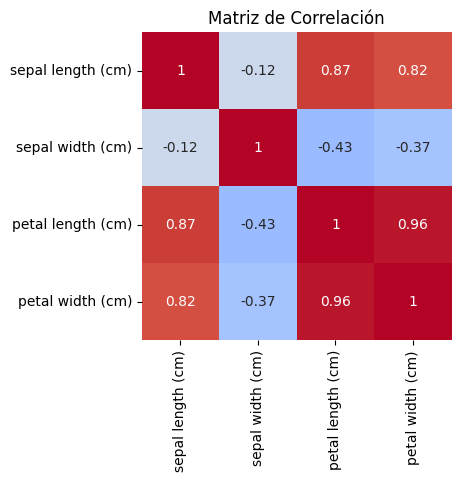
\includegraphics[width = 0.75\textwidth]{Img/heatmap.png}
    \caption{Heatmap de la matriz de Correlación.}
\end{figure}

\subsubsection{Pares de variables con correlación positiva fuerte}

Gracias a la función \texttt{filtro}, pudimos encontrar las variables con correlación fuerte, 
las cuales son las siguientes: 

\begin{itemize}
    \item Longitud de sépalo $\Leftrightarrow$ Longitud de pétalo ($\rho = 0.871$).
    \item Longitud de sépalo $\Leftrightarrow$ Ancho de pétalo ($\rho = 0.817$).
    \item Longitud de pétalo $\Leftrightarrow$ Ancho de pétalo ($\rho = 0.962$).
\end{itemize}

\subsubsection{¿Cómo se relacionan las correlaciones con las diferntes especies?}

Hasta no hacer el análisis correspondiente, no se puede dar una respuesta sólida; solo 
una hipótesis de que la correlación de las distintas medidas de las flores definen las 
especies. 

\QED

\subsubsection{Repetir el análisis anterior por especie}

Para no repetir el proceso tres veces se optó por hacer un diccionario filtrando 
las especies, para después iterar y hacer el respectivo análisis.

Definamos el siguiente diccionario: 

\begin{lstlisting}[language = python, caption = {Diccionario de dataframes.}]
dfs = {especie: datos.iloc[:, 0:4] for especie, datos in df_iris.groupby('species')}
\end{lstlisting}

Procedemos a calcular las matris de correlación y a gaurdarlas en una lista. 

\begin{lstlisting}[language = python, caption = {.}]
matrices_correlacion = []

for i in range(len(dfs)):
    
    matrices_correlacion.append(dfs[i].corr(method = 'pearson'))
\end{lstlisting}

Ahora visualizamos las matrices de correlación de las distintas especies:
\begin{lstlisting}[language = python, caption = {.}]
for i in range(len(dfs)):

    print(f"Matriz de Correlación de la especie {i}")
    
    display(matrices_correlacion[i].round(3))
    print("\n")
\end{lstlisting}

\textbf{Matriz de correlación de la especie 0:}

$$ \mathcal{M}_{\rho_0} =
\begin{bmatrix}
1     & 0.743 & 0.267 & 0.278 \\
0.743 & 1     & 0.178 & 0.233 \\
0.267 & 0.178 & 1     & 0.332 \\
0.278 & 0.233 & 0.332 & 1
\end{bmatrix}
$$

\textbf{Matriz de correlación de la especie 1:}

$$ \mathcal{M}_{\rho_1} =
\begin{bmatrix}
1     & 0.526 & 0.754 & 0.546 \\
0.526 & 1     & 0.561 & 0.664 \\
0.754 & 0.561 & 1     & 0.787 \\
0.546 & 0.664 & 0.787 & 1
\end{bmatrix}
$$

\textbf{Matriz de correlación de la especie 2:}

$$ \mathcal{M}_{\rho_2} = 
\begin{bmatrix}
1     & 0.457 & 0.864 & 0.281 \\
0.457 & 1     & 0.401 & 0.538 \\
0.864 & 0.401 & 1     & 0.322 \\
0.281 & 0.538 & 0.322 & 1
\end{bmatrix}
$$

Ahora aplicaremos la función \texttt{filtro} para encontrar las correlaciones altas de 
cada una de las matrices.

\begin{lstlisting}[language = python, caption = {Correlaciones altas de las matrices.}]
for i in range(len(dfs)):

    print(f'\nRelaciones con correlación alta de la especie {i}:')
    print(filtro(matrices_correlacion[i].round(3), 0.75))
\end{lstlisting}

\begin{lstlisting}[language = python, caption = {Relaciones con correlación alta.}]
Relaciones con correlación alta de la especie 0:
[]

Relaciones con correlación alta de la especie 1:
[('sepal length (cm)', 'petal length (cm)', np.float64(0.754)), ('petal length (cm)', 'petal width (cm)', np.float64(0.787))]

Relaciones con correlación alta de la especie 2:
[('sepal length (cm)', 'petal length (cm)', np.float64(0.864))]
\end{lstlisting}

Finalmente imprimimos cada uno de los heatmaps.

\begin{lstlisting}[language = python, caption = {Heatmaps por especie.}]
plt.figure(figsize = (18, 6))

colores = ['Reds', 'Greens', 'Blues']

for i, (matriz, color) in enumerate(zip(matrices_correlacion, colores)):
    
    plt.subplot(1, 3, i + 1)
    
    sns.heatmap(
        matriz,
        annot = True,
        cmap = color,
        vmin = -1,
        vmax = 1,
        cbar = False
    )
    
    plt.title(f'Matriz de correlación de la especie {i}')

plt.tight_layout()
plt.show()
\end{lstlisting}


\begin{figure}[H]
    \centering
    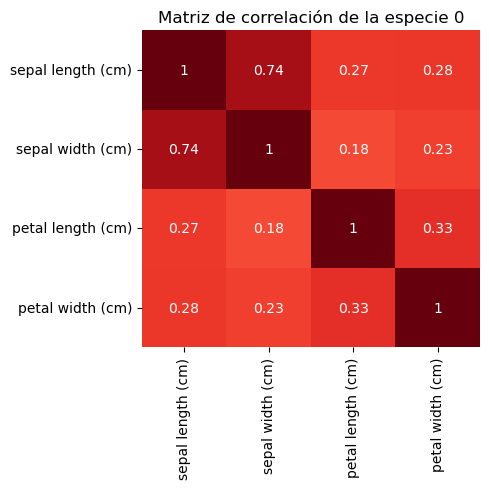
\includegraphics[width = 0.5\textwidth]{Img/heatmap0.png}
    \caption{Heatmap de la especie 0.}
\end{figure}

\begin{figure}[H]
    \centering
    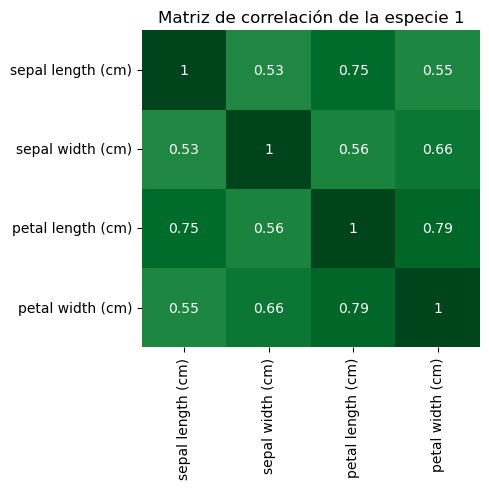
\includegraphics[width = 0.5\textwidth]{Img/heatmap1.png}
    \caption{Heatmap de la especie 1.}
\end{figure}

\begin{figure}[H]
    \centering
    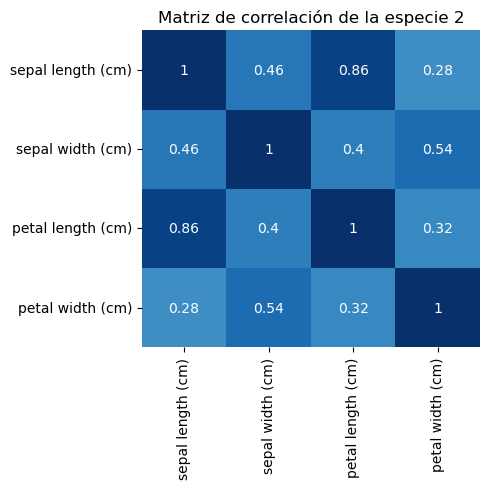
\includegraphics[width = 0.5\textwidth]{Img/heatmap2.png}
    \caption{Heatmap de la especie 2.}
\end{figure}